\onehalfspacing

\section{Model Classification}

\subsection{Training on GENIE Dataset}
\noindent After the training process is complete, the model weights and biases are saved to be able to transfer the results of the training to test the trained model on event samples that the network had not seen during the training and validation process. As well as this, statistics from the training and validation process are produced, giving the accuracy and loss values at each epoch. \medskip

\noindent The accuracy is defined as the fraction of the data set that the model correctly classifies, with respect to the truth label. The output of the model, for each event, is a vector with 3 components, much like the shape of the label that was given to the model, However, the result of the network will not be a one-hot encoded vector, but will have the model's confidence in predicting each class- with the model's predicted class being the that the model is most confident in - the vector component with the largest value. As these values represent probabilities of correct classification, the three components will sum to 1.\medskip

\noindent As the weights of the network as initially randomly generated, one would expect it's initial predictions to be poor. As the model is given more training data it can alter these weights to better fit to the data, and thus one would expect the accuracy of the model to increase over time. Similarly, this means that the loss values are expected to decrease over time.\medskip

\noindent Alongside the training accuracy and loss, the validation accuracy loss are given from the training process. These are the values given testing the model on the validation set- containing data not seen in the training process. This process takes place at the end of each training epoch, and no backpropagation takes place, the model is simply used for inference on the data to produce the accuracy and loss values to judge how the model is performing on unseen data, to see whether it is struggling to fit, overfitting, or successfully fitting to the data. \medskip

\begin{figure}[t!]
 \centering
 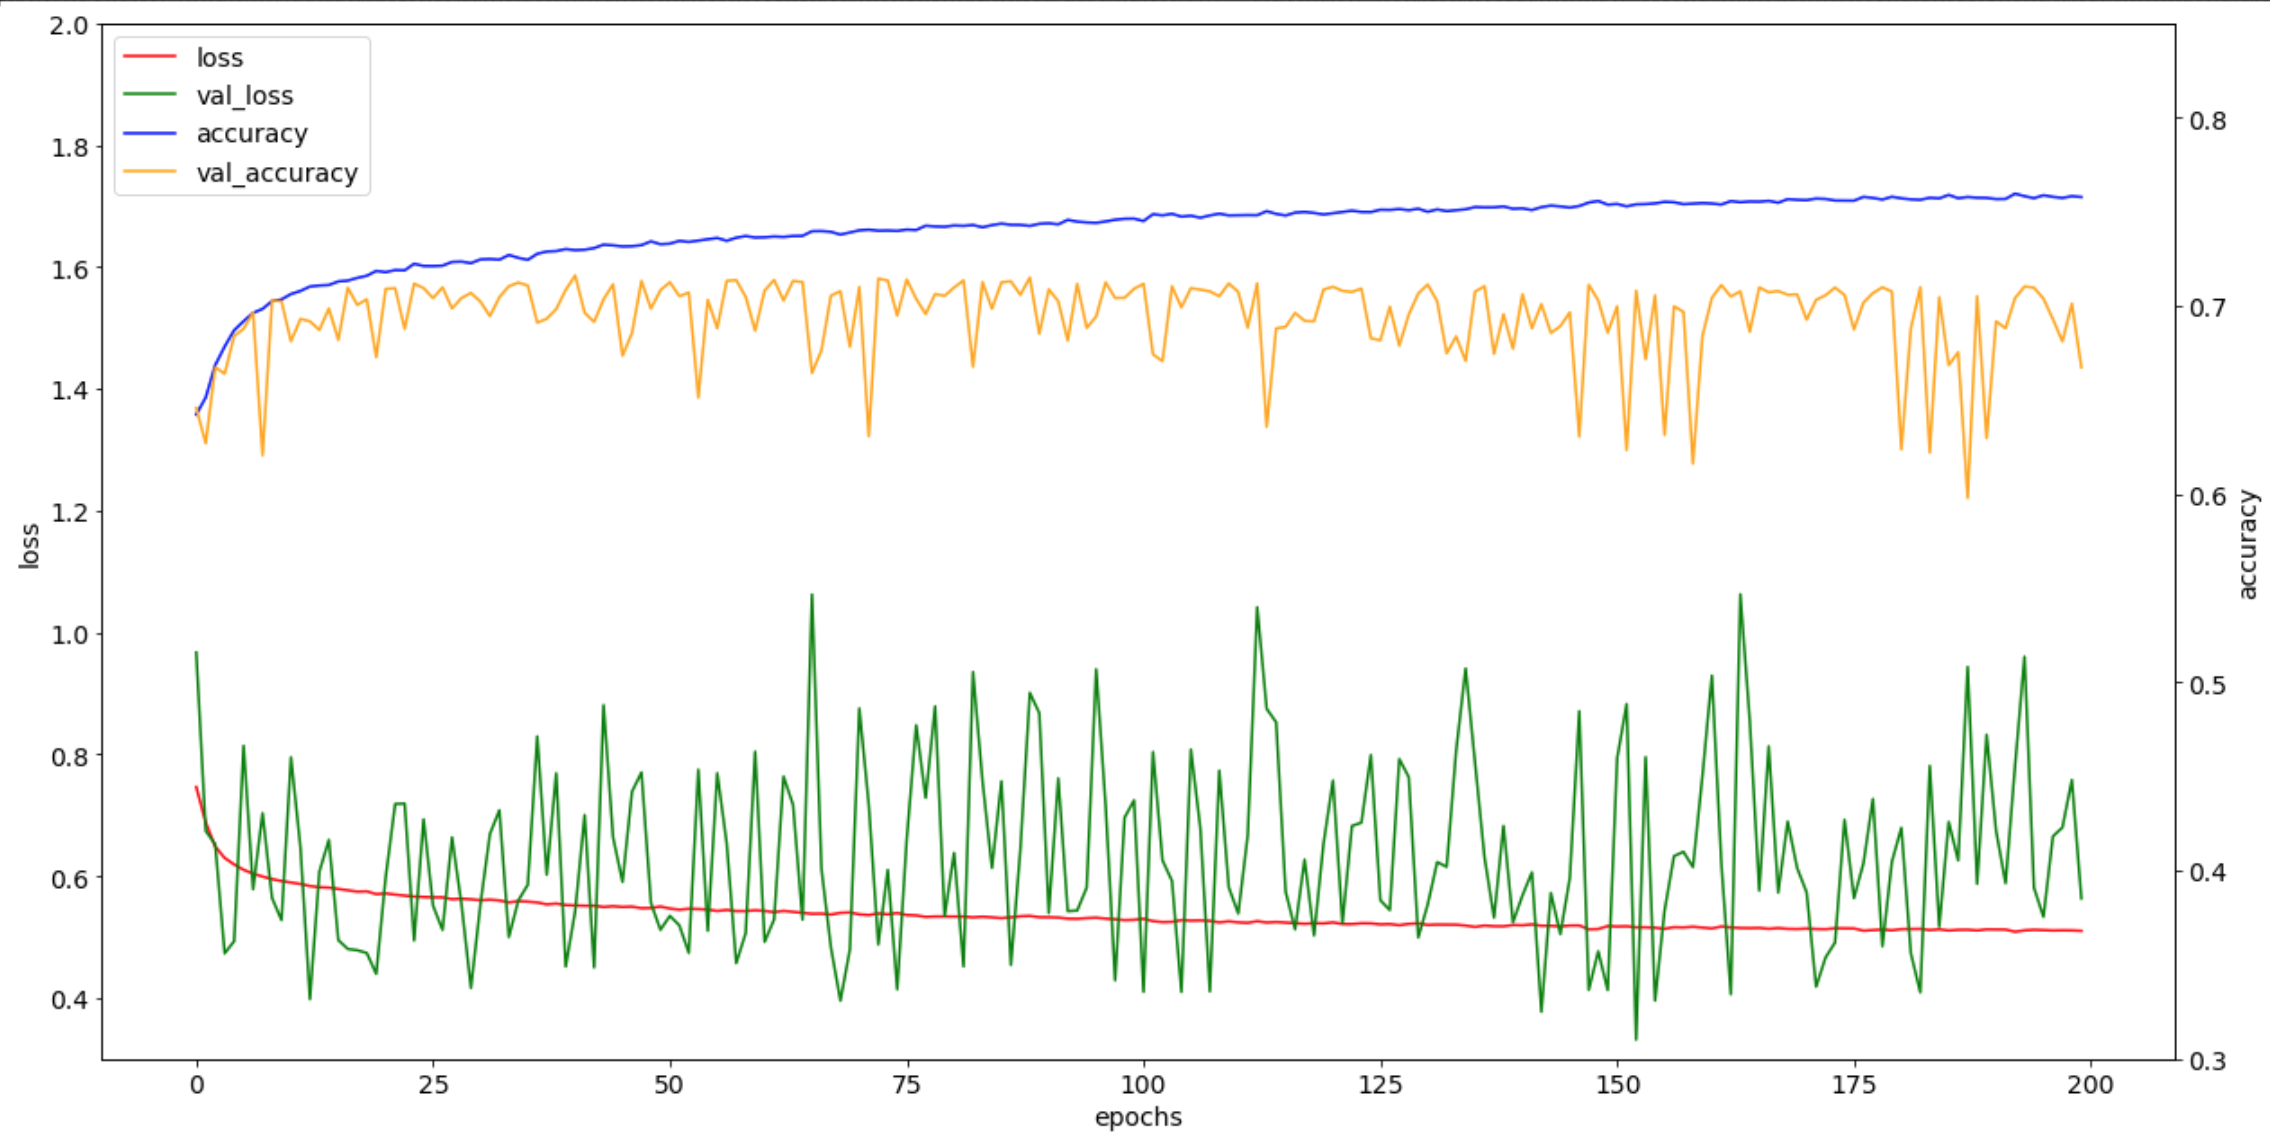
\includegraphics[width=160mm]{genie/acc_loss.png}
 
 \textbf{Figure 9.} \textit{Network training and validation accuracy and loss. The network was trained over 200 epochs using only GENIE generated events. The dateset was not balanced, and the number of $\nu_\mu$ events far exceed that of the other classes. }
\end{figure}

\noindent The MobileNet model was trained on 370864 samples from the GENIE event generator and validated on 52980 samples. The training took place over 200 epochs. As can be seen from the training data, Figure 9, the classifier performs very poorly. The classifier has overfit to the data set, and is struggling to generalise to the unseen validation data, producing the gap between the training accuracy, and the validation accuracy. Unlike traditional overfitting problems where the model overfits by capturing the statistical noise of the data, the overfitting here is taking place due to the data imbalance from the training dataset. In the training dataset, 239932 of the samples were $\nu_\mu$ interactions, 11564 $\nu_e$ interactions, and 119366 NC interactions, and these proportions were mirrored in the validation and testing datasets. Here the classifier can naively predict the event to be a $\nu_\mu$ event every time and be correct 65\% of the time.\medskip

\noindent An ideal classifier will produce two distinct distributions, whereby it can confidently predict the correct classification, and also confidently classify those that are of the the other classes- ie a very low prediction probability of $\nu_e$ or NC events when the truth value is a $\nu_\mu$ event. In Figure 10, it can be seen that a large number of $\nu_\mu$ events are accurately predicted with a high probability, however, the truth $\nu_e$ and NC events are also being classified as $\nu_\mu$ events. This classifier has struggled to determine the differences between the different classes. This can also be seen in Figure 11, where the $\nu_e$ classifier correctly identified $\nu_\mu$ and NC events as not $\nu_e$ events with a high probability, however it is classifying every event as a $\nu_\mu$, and thus no events as $\nu_e$ interactions, and incorrectly classifying the $\nu_e$ events.\medskip

\noindent In this case it is redundant to look at the purity and the efficiency of the classifier as every event is being classifier as as $\nu_\mu$ event, giving the classifier a very high efficiency, as all the $\nu_\mu$ events are identified correctly, however the purity of the classifier is poor as events that are not $\nu_\mu$ events are being classified as so. \medskip

\begin{figure}[t!]
 \centering
 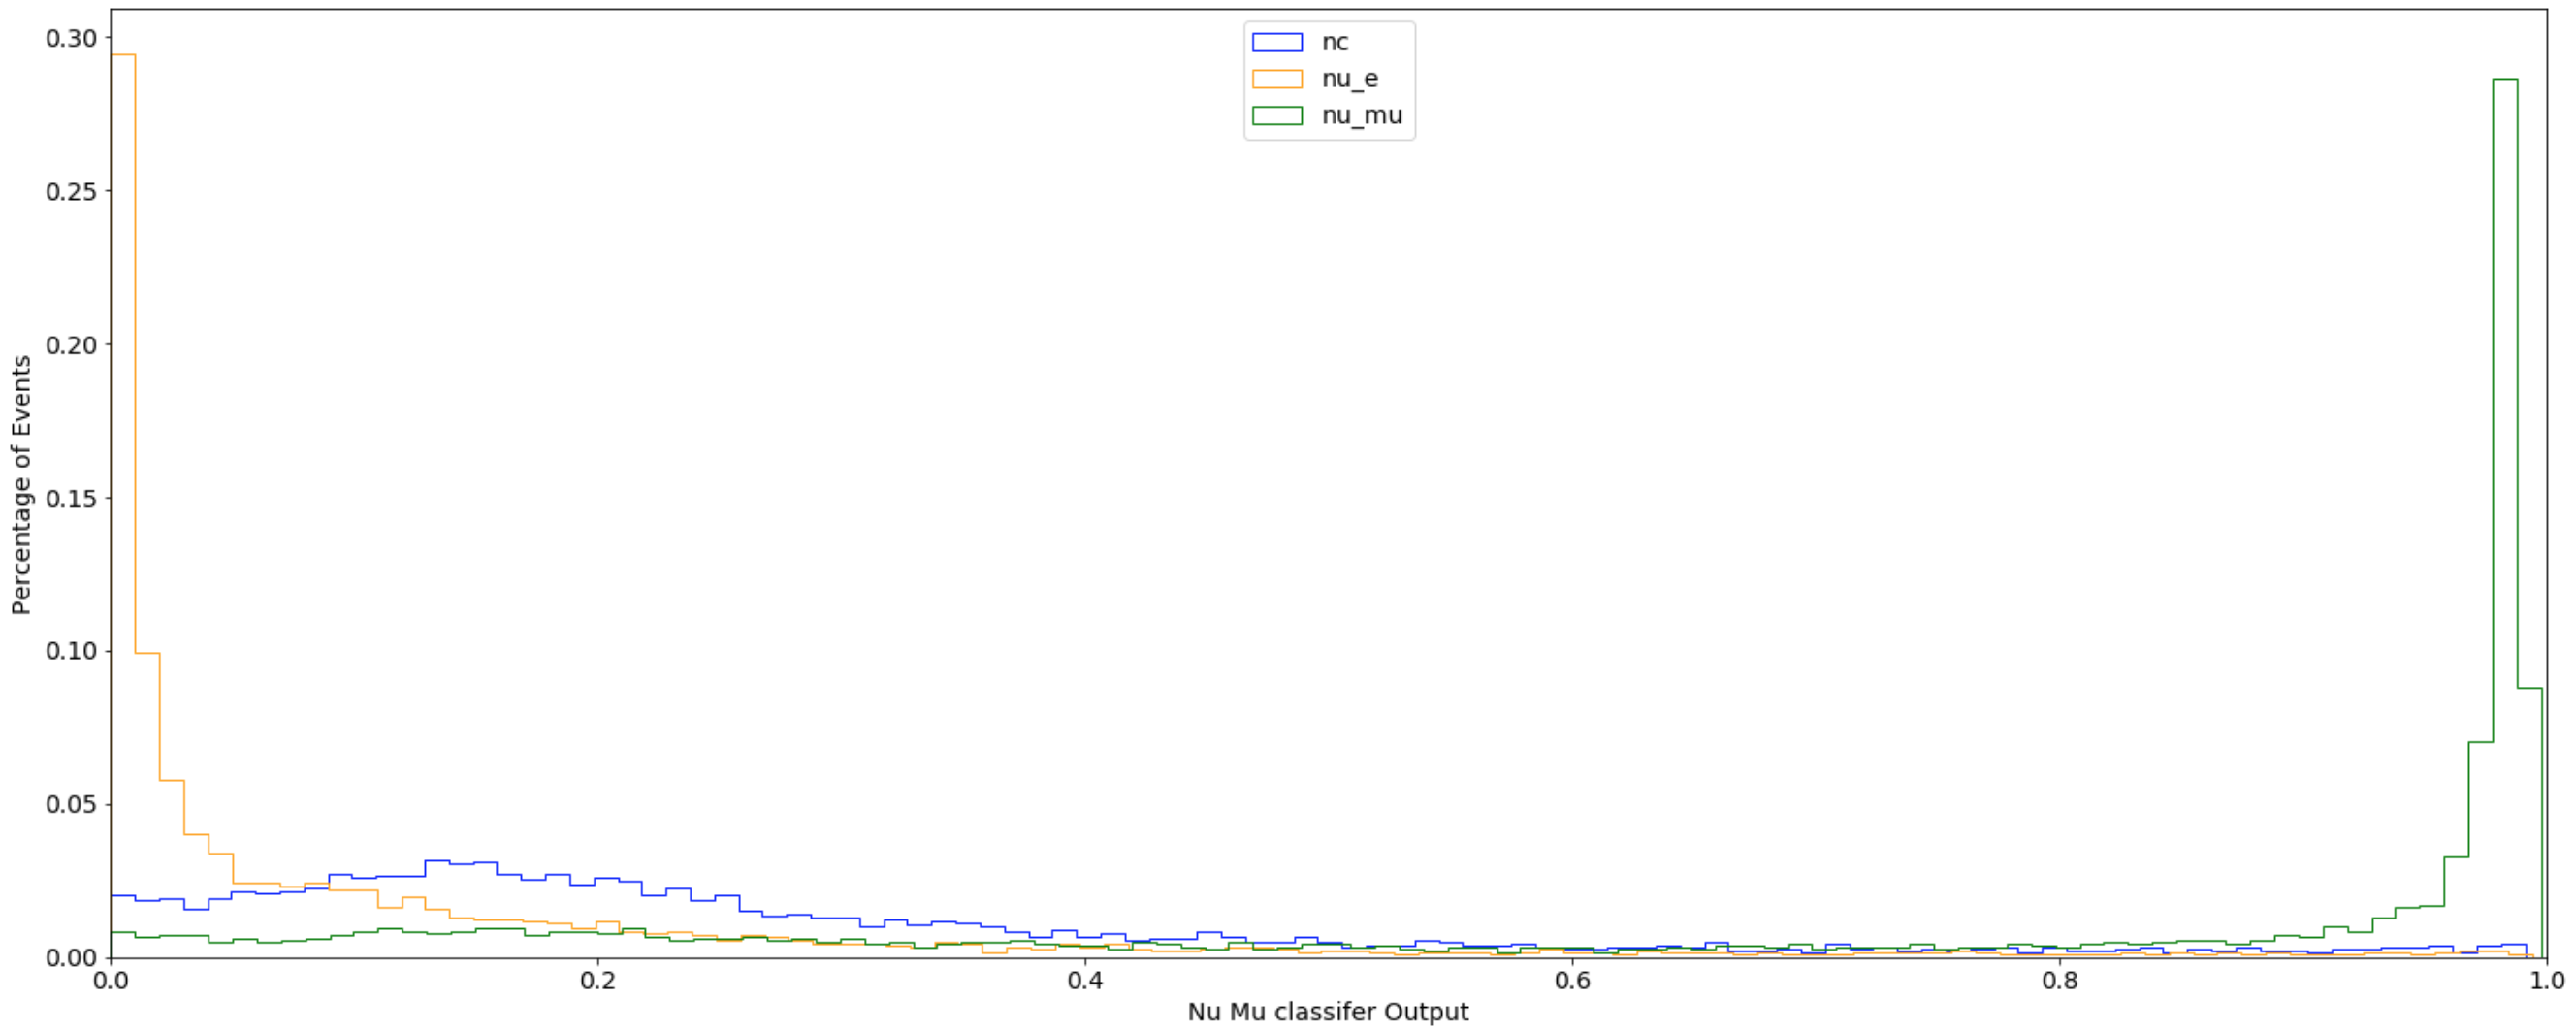
\includegraphics[width=160mm]{genie/NUMU.png}
 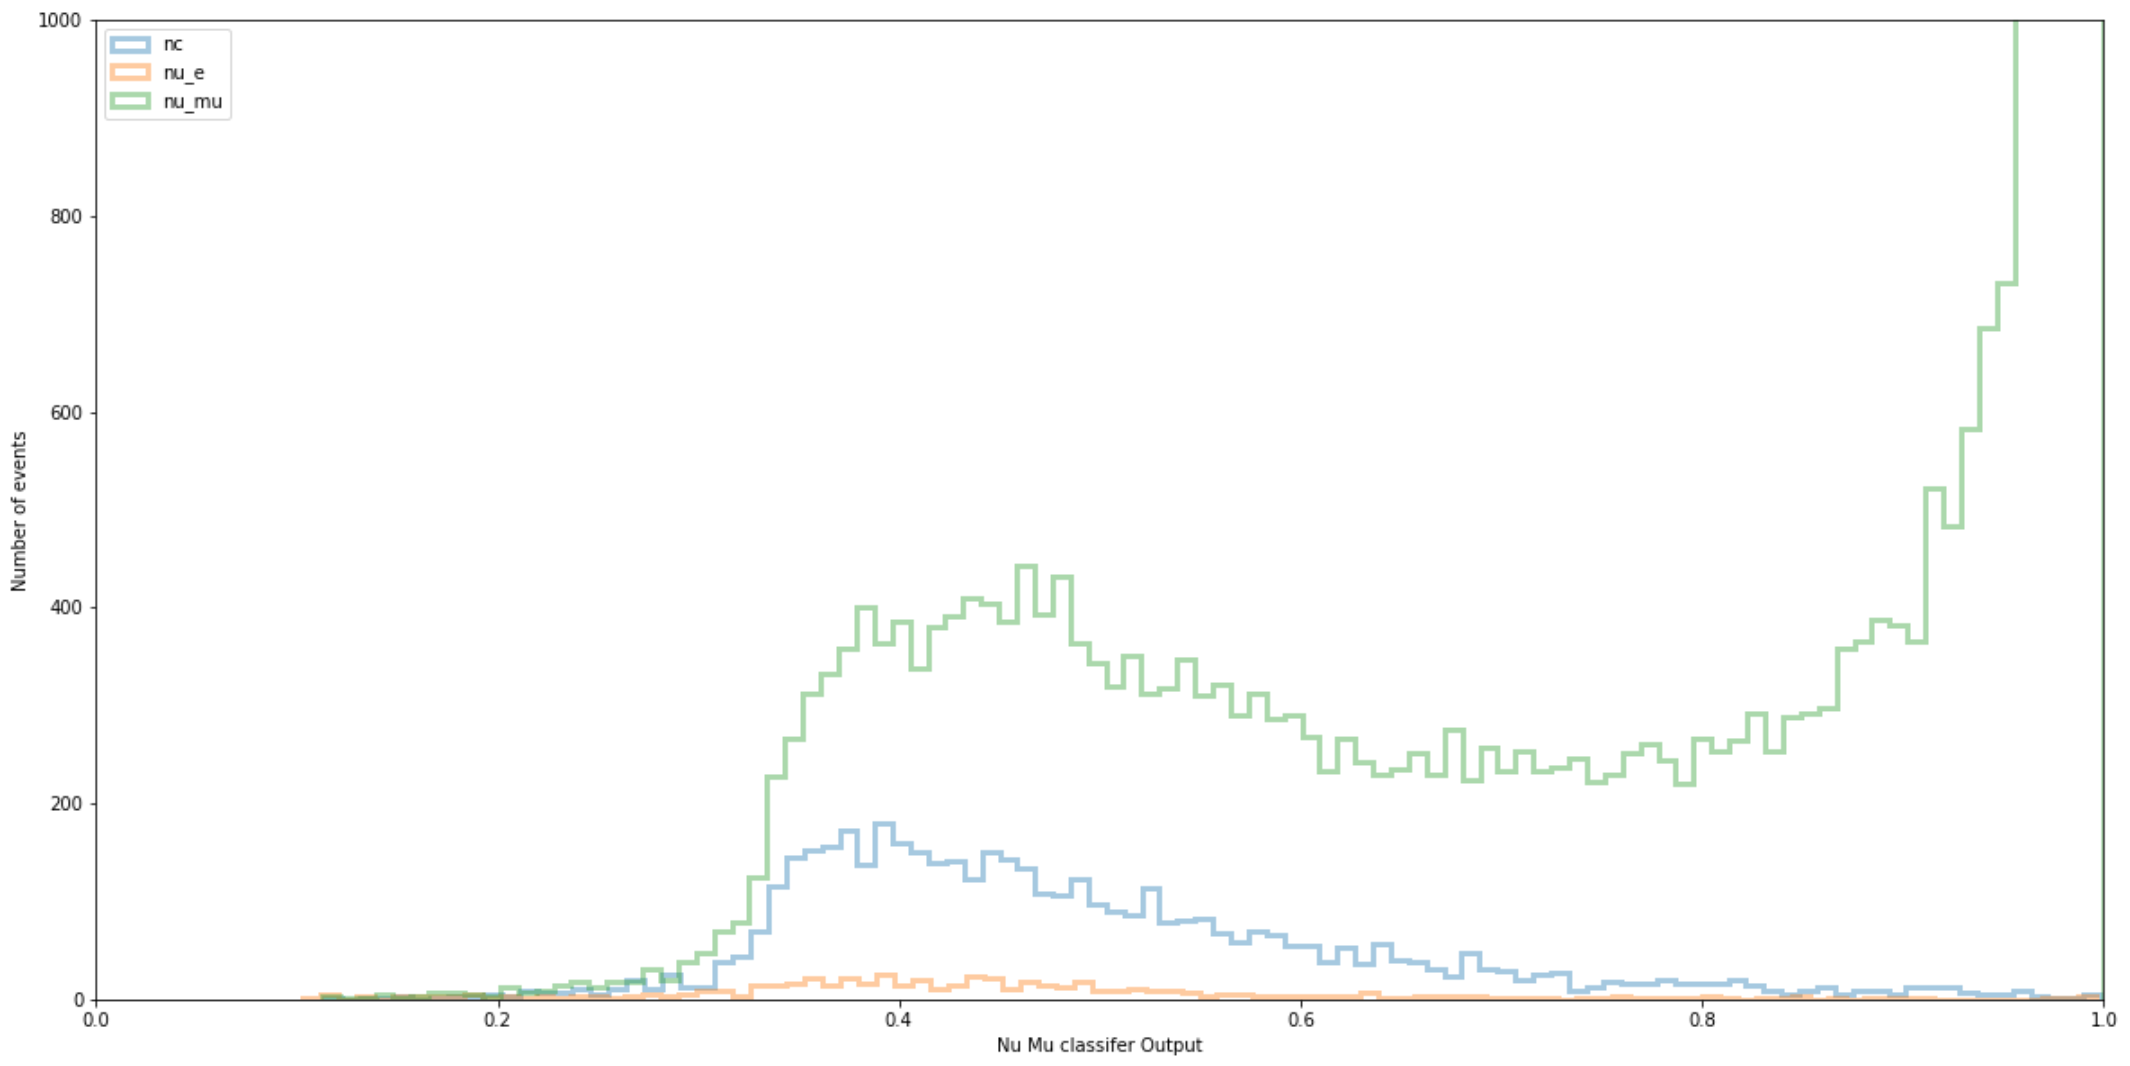
\includegraphics[width=160mm]{genie/NUMUZOOM.png} 
 
 \textbf{Figure 10.} \textit{$\nu_\mu$ classification output histogram. The dataset was trained and tested using only GENIE generated events. The dateset was not balanced, and the number of $\nu_\mu$ events far exceed that of the other classes.  Figures show the probability of being classified a $\nu_\mu$ for events of all the interaction types. Top Figure shows the entire dataset, while the bottom Figure shows a cropped version of the same dataset with the axis limited to a reduced number of counts.}
\end{figure}

\begin{figure}[t!]
 \centering
 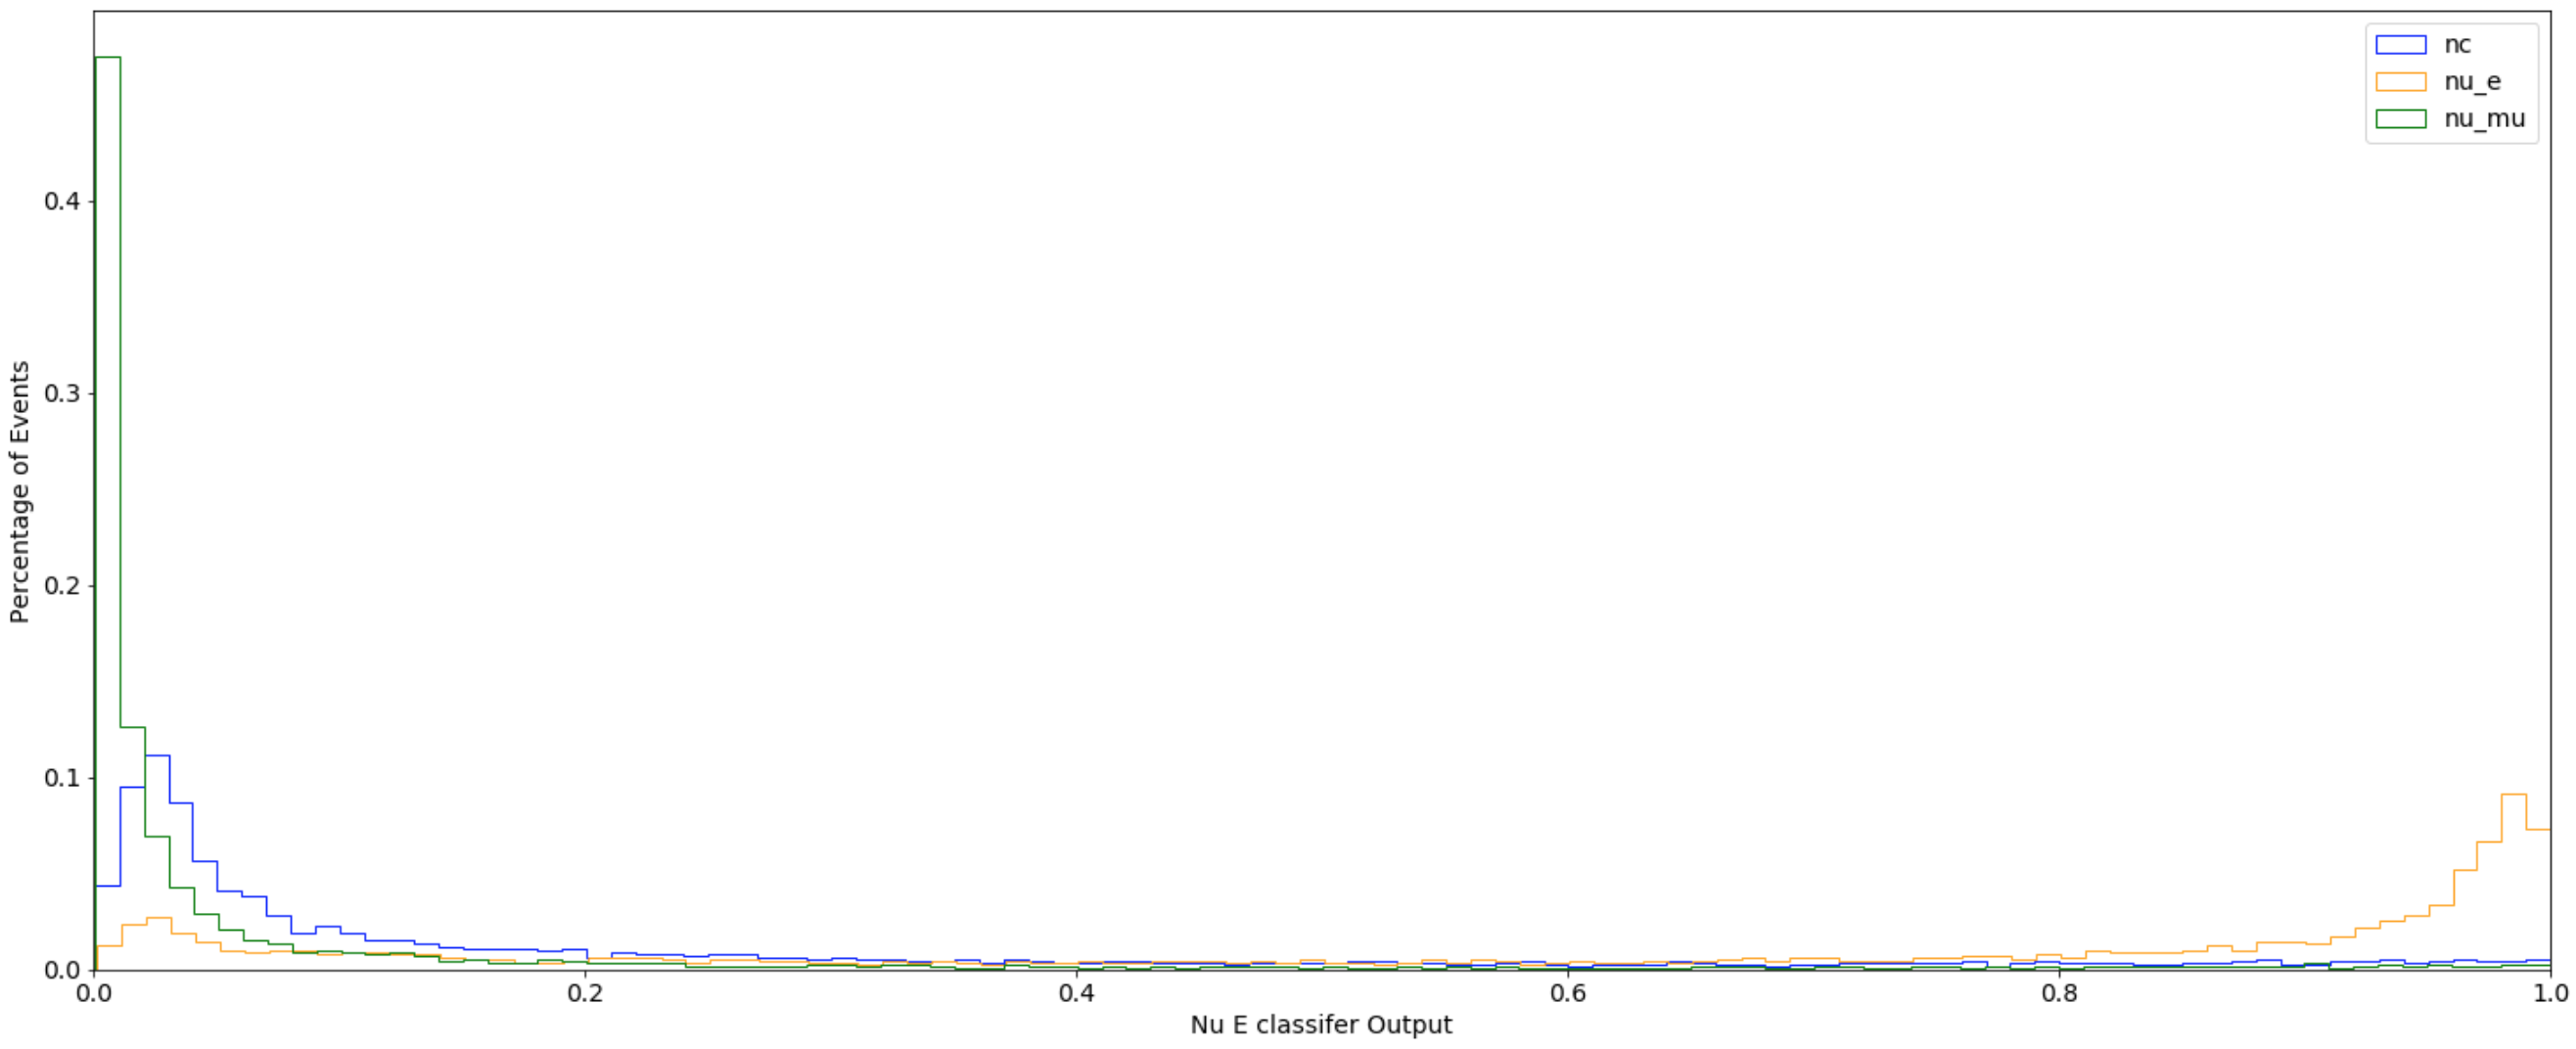
\includegraphics[width=160mm]{genie/NUE.png}
 
 \textbf{Figure 11.} \textit{$\nu_e$ classification output histogram. Figures show the probability of being classified a $\nu_\mu$ for events of all the interaction types. The training process was the same as for that in Figure 10.}
\end{figure}



